\chapter{Taxonomía de SOLO adaptada a la matemática}

{\small\tabcolsep=4.5pt
\begin{longtable}{|l|l|l|l|l|}
% aquí añadimos el encabezado de la primera hoja.
\hline
\rowcolor[HTML]{00C0F3}
\textbf{1. Preestructural} & \textbf{2. Uniestructural} & \textbf{3. Multiestructural} & \textbf{4. Relacional} & \begin{tabular}[c]{@{}l@{}} \textbf{5. Abstracto} \\ \textbf{Ampliado}\end{tabular}\\
\endfirsthead

% aquí añadimos el encabezado del resto de hojas.
\hline
\rowcolor[HTML]{00C0F3} \textbf{1. Preestructural} & \textbf{2. Uniestructural} & \textbf{3. Multiestructural} & \textbf{4. Relacional} & \begin{tabular}[c]{@{}l@{}} \textbf{5. Abstracto} \\ \textbf{Ampliado}\end{tabular} \\ 
\endhead
% aquí añadimos el fondo de todas las hojas, excepto de la última.
\multicolumn{5}{l}{Sigue en la página siguiente.}
\endfoot
% aquí añadimos el fondo de la última hoja.
\endlastfoot
\hline
 & Identificar & Distinguir & Relacionar & Evaluar \\ \hline
\rowcolor[HTML]{8ED8F8} 
 & Nombrar & Comparar & Modelar & Modelar \\ \hline
 & Definir & \begin{tabular}[c]{@{}l@{}}Aplicar: algoritmos, \\ teoremas, \\ definiciones\end{tabular} & Comparar & Formular \\ \hline
\rowcolor[HTML]{8ED8F8} 
 & \begin{tabular}[c]{@{}l@{}}Seguir instrucciones \\ simples\end{tabular} & Listar & Contrastar & Teorizar \\ \hline
 & \begin{tabular}[c]{@{}l@{}}Realizar cálculos \\ básicos: calcular,\\ graficar, simplificar,\\  operar, etc\end{tabular} & Combinar & Asociar & Predecir \\ \hline
\rowcolor[HTML]{8ED8F8} 
 & \begin{tabular}[c]{@{}l@{}}Resolver: ecuaciones\\ e inecuaciones \\ sencillas, problemas\\  sencillos, etc\end{tabular} & Calcular & Analizar & Crear \\ \hline
 & \begin{tabular}[c]{@{}l@{}}Reproducir \\ procedimientos \\ básicos: factorizar,\\ resolver ecuaciones,\\ graficar, calcular\end{tabular} & \begin{tabular}[c]{@{}l@{}}Realizar cálculos más \\ elaborados: optimizar\\ (en una y varias \\ variables), calcular \\ determinantes, \\ integrar, resolver \\ sistemas de\\ ecuaciones lineales\end{tabular} & Demostrar & Imaginar \\ \hline
\rowcolor[HTML]{8ED8F8} 
 & \begin{tabular}[c]{@{}l@{}}Efectuar tareas \\ sencillas: calcular,\\ hacer construcciones\\ gráficas, buscar \\ lugares geométricos,\\ resolver ecuaciones,\\ derivar, integrar, etc.\end{tabular} & \begin{tabular}[c]{@{}l@{}}Demostrar resultados \\ simples: \\ demostraciones\\ de caracter operacional, \\ verificaciones básicas, \\ dar ejemplos y \\ contraejemplos.\end{tabular} & Experimentar & Hipotetizar \\ \hline
 & Argumentar &  & Argumentar & Generalizar \\ \hline
\rowcolor[HTML]{8ED8F8} 
 & Ejemplificar & \begin{tabular}[c]{@{}l@{}}Experimentar: con y sin \\ recursos \\ computacionales como \\ software\end{tabular} & Justificar & Reflejar \\ \hline
 & Calcular & \begin{tabular}[c]{@{}l@{}}Reproducir \\ procedimientos\\ elaborados: integrar, \\ ortonormalizar (Gram-\\ Schmidt), diagonalizar\end{tabular} & Criticar & Demostrar \\ \hline
\rowcolor[HTML]{8ED8F8} 
 & Determinar: valores & Argumentar & Interpretar & Experimentar \\ \hline
 & \begin{tabular}[c]{@{}l@{}}Ejecutar: comandos\\ de software \\ (Wolfram Alpha,\\ Mathematica)\end{tabular} & Ejemplificar & \begin{tabular}[c]{@{}l@{}}Programar:\\ algoritmos, rutinas,\\ etc, para resolver\\ problemas \\ complejos\end{tabular} & Explicar \\ \hline
\rowcolor[HTML]{8ED8F8} 
 &  & \begin{tabular}[c]{@{}l@{}}Implementar: \\ algoritmos \\ básicos en software\end{tabular} & \begin{tabular}[c]{@{}l@{}}Implementar:\\ algoritmos, \\ rutinas\end{tabular} & Justificar \\ \hline
 &  & \begin{tabular}[c]{@{}l@{}}Elaborar: documentos \\ científicos en LaTeX, \\ Beamer, informes,\\ reportes, etc.\end{tabular} & Indagar & Conjeturar \\ \hline
\rowcolor[HTML]{8ED8F8} 
 &  &  &  & Visualizar \\ \hline
 &  &  &  & Interpretar \\ \hline
\rowcolor[HTML]{8ED8F8} 
 &  &  &  & \begin{tabular}[c]{@{}l@{}}Desarrollar:\\ algoritmos, \\ modelos, etc\end{tabular} \\ \hline
 &  &  &  & Investigar \\ \hline
\end{longtable}
}

\chapter{Gestión curricular}
En este apartado se plantea componentes necesarios para la administración educativa de la malla curricular, incluyendo el plan de transición para estudiantes activos del plan de estudios vigente. También se aborda la evaluación curricular posterior a su futura implementación y la forma en que el personal docente será capacitado a las nuevas exigencias de la malla curricular.

\section{Administración y ejecución}

\subsection{Estructura administrativa de la unidad académica}

La carrera Bachillerato y Licenciatura en Matemática pertenece al Departamento de Matemática y Ciencias Actuariales, el cual actualmente administra también la carrera Bach. y Lic. en Ciencias Actuariales. En la Figura \ref{fig:dpto} se presenta la estructura administrativa vigente. Actualmente existe una solicitud para crear el Departamento de Ciencias Actuariales, con lo que se espera que el Departamento de Matemática y Ciencias Actuariales se convierta en el Departamento de Matemática, a cargo exclusivamente de la carrera de Matemática. Esto permitirá un enfoque especializado en temas de plan de estudios, investigación, acción social y apoyo a estudiantes, buscando potenciar ambas carreras a nivel nacional e internacional. Además, en eventuales procesos de autoevaluación y acreditación, cada departamento podrá concentrar esfuerzos en cada carrera específica.

\begin{figure}
    \centering
    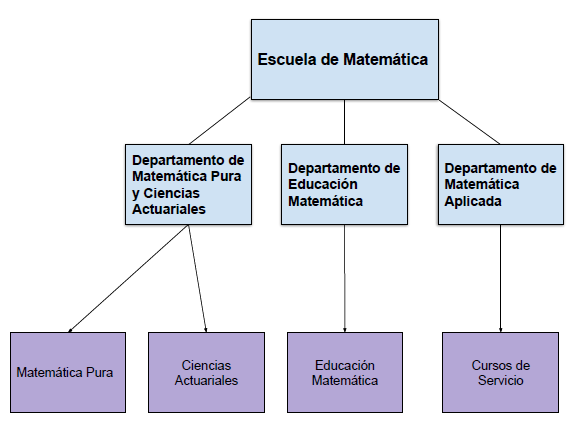
\includegraphics[width=0.5\linewidth]{dptos.png}
    \caption{División por departamentos vigente en la Escuela de Matemática}
    \label{fig:dpto}
\end{figure}

\subsection{Cuerpo docente}
En la Tabla \ref{tab:docentes} se presenta el personal docente activo que ha impartido cursos en la carrera de Matemática desde el año 2010. Se clasifican por áreas de especialización, que corresponde a la especialización que tiene más cercanía a las áreas curriculares que se definieron con anterioridad. En la última columna de la tabla se especifica si el nombramiento de cada docente es en propiedad (P), becario (B), exbecario (E), o interinazgo (I).

% Please add the following required packages to your document preamble:
% \usepackage{longtable}
% Note: It may be necessary to compile the document several times to get a multi-page table to line up properly
\begin{longtable}[c]{|l|l|c|}
\caption{Lista de docentes en condición activa que han impartido cursos desde el 2010.}
\label{tab:docentes}\\
\hline
\rowcolor[HTML]{00C0F3}
Docente & Especialidad & Nombramiento \\ \hline
%
\endhead
%
Jennifer Acuña Larios & Análisis & P \\ \hline
Luis Acuña Valverde &  & P \\ \hline
Josué Ávila Artavia &  & E \\ \hline
Luis Barboza Chinchilla &  & P \\ \hline
Adrián Barquero Sánchez &  & P \\ \hline
Raúl Bolaños Guerrero &  & P \\ \hline
Ronald Bustamante Medina &  & P \\ \hline
Juan Gabriel Calvo Alpízar &  & P \\ \hline
Santiago Cambronero Villalobos &  & P \\ \hline
José David Campos Fernández &  & P \\ \hline
Daniel Campos Salas &  & P \\ \hline
Santiago Chaves Aguilar &  & E \\ \hline
Pedro Díaz Navarro &  & I \\ \hline
Christian Fonseca Mora &  & P \\ \hline
Álvaro Guevara Villalobos &  & P \\ \hline
Jorge Guier Acosta &  & P \\ \hline
Jonathan Gutiérrez Pavón &  & P \\ \hline
Alberto Hernández Alvarado &  & P \\ \hline
David Jiménez López &  & P \\ \hline
David Krumm Cabezas &  & I \\ \hline
Allan Lacy Mora &  & P \\ \hline
Jennifer Loría Sorio &  & E \\ \hline
Darío Mena Arias &  & P \\ \hline
Pedro Méndez Hernández &  & P \\ \hline
Carlos Montalto Cruz &  & P \\ \hline
Samaria Montenegro Guzmán &  & P \\ \hline
German Mora Sáenz &  & B \\ \hline
Adrián Naranjo Alvarado &  & B \\ \hline
Hugo Peña Gómez &  & I \\ \hline
Alexander Ramírez González &  & P \\ \hline
Oldemar Rodríguez Rojas &  & P \\ \hline
José Rosales Ortega &  & P \\ \hline
Adriana Sánchez Chavarría &  & P \\ \hline
Jesús Sánchez Guevara &  & P \\ \hline
Fabio Sánchez Peña &  & P \\ \hline
Esteban Segura Ugalde &  & P \\ \hline
Filánder Sequeira Chavarría &  & I \\ \hline
Maikol Solís Chacón &  & P \\ \hline
Javier Trejos Zelaya &  & P \\ \hline
William Ugalde Gómez &  & P \\ \hline
Roberto Ulloa Esquivel &  & E \\ \hline
Mario Villalobos Arias &  & P \\ \hline
Mark Villarino Bertran &  & P \\ \hline
Rafael Zamora Calero &  & P \\ \hline
Óscar Zamora Luna &  & E \\ \hline
Ronald Zúñiga Rojas &  & P \\ \hline
\end{longtable}


Con base en la información anterior, se detalla la cantidad de profesores disponibles (no exclusivos) por cada uno de los cursos que componen la malla curricular propuesta en la Tabla \ref{tab:cursos}. Es importante agregar que muchos docentes están simultáneamente disponibles en más de un curso, por lo que esta tabla representa un escenario optimista de la cantidad de recursos disponibles en la Escuela de Matemática para hacerle frente a la oferta académica. Cada curso se espera que sea impartido por docentes con doctorado. En el caso de tener maestría, se permitirá si el  curso es relacionado con el área de trabajo. %Por otro lado, la columna que indica el grado académico mínimo es definido con respecto a la complejidad de los contenidos y a la ubicación del curso en la malla curricular.


\begin{longtable}[c]{|l|p{7cm}|p{3.4cm}|p{2cm}|}
\caption{Número de personal docente por curso del nuevo plan de estudios, según especialidad}
\label{tab:cursos}\\
\hline
\rowcolor[HTML]{00C0F3}
Sigla & Curso & Área de especialidad & Número de docentes \\ \hline
%
\endhead
%
\MA{0151} & \gls{MA0151} & General &  \\ \hline
\MA{0152} & \gls{MA0152} & General &  \\ \hline
\MA{0251} & \gls{MA0251} & General &  \\ \hline
\MA{0252} & \gls{MA0252} & General &  \\ \hline
\MA{0261} & \gls{MA0261} & Álgebra &  \\ \hline
\MA{0341} & \gls{MA0341} & Numérico &  \\ \hline
\MA{0351} & \gls{MA0351} & Análisis &  \\ \hline
\MA{0361} & \gls{MA0361} & Álgebra &  \\ \hline
\MA{0451} & \gls{MA0451} & Análisis &  \\ \hline
\MA{0461} & \gls{MA0461} & Teoría de números &  \\ \hline
\MA{0471} & \gls{MA0471} & Análisis &  \\ \hline
\MA{0472} & \gls{MA0472} & Geometría &  \\ \hline
\MA{0515} & \gls{MA0515} & Análisis &  \\ \hline
\MA{0520} & \gls{MA0520} & Análisis/Estadística &  \\ \hline
\MA{0535} & \gls{MA0535} & Álgebra &  \\ \hline
\MA{0541} & \gls{MA0541} & Numérico &  \\ \hline
\MA{0615} & \gls{MA0615} & Análisis &  \\ \hline
\MA{0625} & \gls{MA0625} & Análisis &  \\ \hline
\MA{0635} & \gls{MA0635} & Álgebra &  \\ \hline
\MA{063X} & \gls{MA063X} & Topología &  \\ \hline
\MA{0702} & \gls{MA0702} & Análisis &  \\ \hline
\MA{0725} & \gls{MA0725} & Análisis &  \\ \hline
\MA{07xx} & \gls{MA07xx} & Geometría &  \\ \hline
\MA{-OPT} & \gls{OPT-Algebra} & Álgebra &  \\ \hline
\MA{-OPT} & \gls{OPT-Analisis} & Análisis &  \\ \hline
\MA{-OPT} & \gls{OPT-Aplicada} & Aplicada &  \\ \hline
\MA{-OPT} & \gls{OPT-Computacion cientifica} & Numérico &  \\ \hline
\MA{-OPT} & \gls{OPT-Discreta} & Discreta &  \\ \hline
\MA{-OPT} & \gls{OPT-Estadistica, Ciencia datos} & Estadística&  \\ \hline
\MA{-OPT} & \gls{OPT-Geometria} & Geometría &  \\ \hline
\MA{-OPT} & \gls{OPT-Logica} & Lógica &  \\ \hline
\MA{-OPT} & \gls{OPT-Topologia} & Topología &  \\ \hline
%\end{tabular}
\end{longtable}


\subsection{Plan de Transición}
Para estudiantes activos que ingresaron en el año 2025 o anteriores, se propone un plan de transición con base en el cohorte que corresponda, bajo el supuesto de que cada estudiante tiene el año correspondiente al cohorte completo al finalizar el año 2025. 

\subsubsection{Cohorte C5}
Se estima que este grupo tendrá 50 estudiantes, quienes aprobaron MA0150 y MA0250, además de los cursos de generales de primer año. A este grupo se le debe convalidar MA0251, MA0252 y permitir que MA0261 sea correquisito con los cursos del I26, como excepción por el plan de transición.
\begin{table}[h!]
\centering
\begin{tabular}{|c|l|}
\hline
\rowcolor[HTML]{00C0F3}
Cohorte C5 & Primer año completo del plan anterior \\ \hline
I26 & \begin{tabular}[c]{@{}l@{}}MA0261 \gls{MA0261} (3)\\ MA0341 \gls{MA0341} (4)\\ MA0351 \gls{MA0351} (4)\\ Artística (2)\end{tabular} \\ \hline
II26 & \begin{tabular}[c]{@{}l@{}}MA0361 \gls{MA0361} (4)\\ MA0451 \gls{MA0451} (4)\\ MA0461 \gls{MA0461} (4)\\ MA0471 \gls{MA0471} (4)\\ Seminario de Realidad Nacional I (2)\end{tabular} \\ \hline
I27 & Igual que Ciclo V - Plan 26 \\ \hline
II 27 & Igual que Ciclo VI - Plan 26 \\ \hline
I 28 & Igual que Ciclo VII - Plan 26 \\ \hline
II 28 & Igual que Ciclo VIII - Plan 26 \\ \hline
\end{tabular}
\end{table}

\subsubsection{Cohorte C4}
Se estima que este grupo tendrá 35 estudiantes, quienes aprobaron MA0150, MA0250, MA0350, MA0360, MA0370, MA0450 y MA0460. A este grupo se le debe convalidar MA0252, MA0351, MA0341, y permitir que MA0461 y MA0535 sean correquisitos, como excepción por el plan de transición.

\begin{table}[h!]
\centering
\begin{tabular}{|l|l|}
\hline
\rowcolor[HTML]{00C0F3}
Cohorte C4 & Segundo año completo del plan anterior) \\ \hline
I26 & \begin{tabular}[c]{@{}l@{}}MA0461 \gls{MA0461} (4)\\ MA0520 \gls{MA0520} (4)\\ MA0535 \gls{MA0535} (4)\\ MA0541 \gls{MA0541} (4)\\ Seminario de Realidad Nacional II (2)\end{tabular} \\ \hline
II26 & Igual que Ciclo VI - Plan 26 \\ \hline
I27 & Igual que Ciclo VII - Plan 26 \\ \hline
II 27 & Igual que Ciclo VIII - Plan 26 \\ \hline
\end{tabular}
\end{table}

\subsubsection{Cohorte C3}
Quienes tengan tres años completos del plan anterior, deben finalizar dicho plan, para lo cual deben cursar MA0702, MA0704, MA0870 y tres optativas de Matemática.

\subsubsection{Excepciones}
Cada estudiante que no haya cumplido sus ciclos de estudio de acuerdo con el plan de estudios anterior, no contemplados en los incisos anteriores, o aquellos de planes previos, deberá de utilizar la tabla de convalidaciones para trasladarse hacia la malla del nuevo plan de estudios, y deberá cursar los cursos no convalidables hasta cumplir con todos los requisitos del plan 2026. 

\subsubsection{Convalidaciones}

Se plantea considerar las siguientes convalidaciones, para casos particulares que no cumplen con un cohorte específico; ver Tabla \ref{tab:conv}. De esta forma, se deberán trasladar al plan 2026, realizando las convalidaciones que correspondan, y deberán cursar aquellos cursos no convalidables hasta cumplir con todos los requisitos del plan 2026.

\begin{table}[h!]
\centering
\caption{Convalidaciones para transicione de plan de estudios}
\label{tab:conv}
\begin{tabular}{|p{6cm}|p{8.5cm}|}
\rowcolor[HTML]{00C0F3}
\hline
Sigla y curso aprobado & Sigla y curso por convalidar \\ \hline
MA0150 Principios de Matematica & \begin{tabular}[c]{@{}l@{}}MA0152 \gls{MA0152}\\ MA0252 \gls{MA0252}\end{tabular} \\ \hline
\begin{tabular}[c]{@{}l@{}}MA0250 Cálculo en una variable I\\ MA0350 Cálculo en una variable II\end{tabular} & \begin{tabular}[c]{@{}l@{}}MA0251 \gls{MA0251}\\ MA0451 \gls{MA0451}\end{tabular} \\ \hline
MA0450 Cálculo en varias variables & \begin{tabular}[c]{@{}l@{}}MA0351 \gls{MA0351}\\ MA0515 \gls{MA0515}\end{tabular} \\ \hline
MA0360 Álgebra lineal I & MA0261 \gls{MA0261} \\ \hline
MA0455 Ec. dif. ordinarias & MA0615 \gls{MA0615} \\ \hline
MA0460 Álgebra lineal II & MA0361 \gls{MA0361} \\ \hline
MA0501 Análisis numérico I & MA0541 \gls{MA0541} \\ \hline
MA0505 Análisis I & MA0625 \gls{MA0625} \\ \hline
MA0561 Grupos y anillos & MA0535 \gls{MA0535} \\ \hline
MA0605 Análisis II & MA0725 \gls{MA0725} \\ \hline
MA0660 Teoría de Galois & MA0635 \gls{MA0635} \\ \hline
MA0704 Topología General I & MA063X \gls{MA063X} \\ \hline
\end{tabular}
\end{table}

\subsection{Proyección de carga académica para el plan de transición}

Según el plan descrito en la sección anterior, se presenta la proyección de carga académica necesaria para suplir la demanda de los años de transición (2026, 2027, 2028). Esto bajo el supuesto de recibir el máximo de 26 estudiantes por año más doce estudiantes por traslado, ofertando dos grupos por curso en primer año.

\begin{longtable}[c]{|l|l|l|l|l|l|}
\caption{Proyección de carga académica para el plan de transición, año 2026}
\label{tab:carga2026}\\
\hline
\rowcolor[HTML]{00C0F3}
Ciclo & Cohorte & Curso & Créditos & Grupos & Jornada \\ \hline
\endhead
%
I & C3 & MA0702 & 5 & 1 & 0.375 \\ \hline
I & C3 & MA0704 & 5 & 1 & 0.375 \\ \hline
I & C3 & MA OPT & 5 & 1 & 0.375 \\ \hline
I & C4 & MA0461 & 4 & 1 & 0.375 \\ \hline
I & C4 & MA0520 & 4 & 1 & 0.375 \\ \hline
I & C4 & MA0535 & 4 & 1 & 0.375 \\ \hline
I & C4 & MA0541 & 4 & 1 & 0.375 \\ \hline
I & C5 & MA0261 & 3 & 1 & 0.375 \\ \hline
I & C5 & MA0341 & 4 & 1 & 0.375 \\ \hline
I & C5 & MA0351 & 4 & 1 & 0.375 \\ \hline
I & C6 & MA0151 & 3 & 2 & 0.375 \\ \hline
I & C6 & MA0152 & 3 & 2 & 0.375 \\ \hline
I & C6 & Inglés I & 3 & 2 & 0.250 \\ \hline
 &  & 14 3/8 & 2 2/8 & Total & 5.750 \\ \hline
II & C3 & MA0870 & 5 & 1 & 0.375 \\ \hline
II & C3 & MA OPT & 5 & 1 & 0.375 \\ \hline
II & C3 & MA OPT & 5 & 1 & 0.375 \\ \hline
II & C4 & MA063X & 4 & 1 & 0.375 \\ \hline
II & C4 & MA0615 & 4 & 1 & 0.375 \\ \hline
II & C4 & MA0625 & 4 & 1 & 0.375 \\ \hline
II & C4 & MA0635 & 4 & 1 & 0.375 \\ \hline
II & C4 & Módulo 1 & 2 & 1 & 0.250 \\ \hline
II & C5 & MA0361 & 4 & 1 & 0.375 \\ \hline
II & C5 & MA0451 & 4 & 1 & 0.375 \\ \hline
II & C5 & MA0461 & 4 & 1 & 0.375 \\ \hline
II & C5 & MA0471 & 4 & 1 & 0.375 \\ \hline
II & C6 & MA0251 & 3 & 2 & 0.375 \\ \hline
II & C6 & MA0252 & 3 & 2 & 0.375 \\ \hline
II & C6 & MA0261 & 3 & 2 & 0.375 \\ \hline
II & C6 & Inglés II & 3 & 2 & 0.250 \\ \hline
 &  & 17 3/8 & 3 2/8 & Total & 7.125 \\ \hline
\end{longtable}

% Please add the following required packages to your document preamble:
% \usepackage{longtable}
% Note: It may be necessary to compile the document several times to get a multi-page table to line up properly
\begin{longtable}[c]{|l|l|l|l|l|l|}
\caption{Proyección de carga académica para el plan de transición, año 2027}
\label{tab:carga2027}\\
\hline
\rowcolor[HTML]{00C0F3}
Ciclo & Cohorte & Curso & Créditos & Grupos & Jornada \\ \hline
\endhead
%
I & C4 & Módulo 2 & 2 & 1 & 0.250 \\ \hline
I & C4 & MA07XX & 4 & 1 & 0.375 \\ \hline
I & C4 & MA0702 & 4 & 1 & 0.375 \\ \hline
I & C4 & MA0725 & 4 & 1 & 0.375 \\ \hline
I & C4 & MA OPT & 4 & 1 & 0.375 \\ \hline
I & C5 & MA0515 & 4 & 1 & 0.375 \\ \hline
I & C5 & MA0520 & 4 & 1 & 0.375 \\ \hline
I & C5 & MA0535 & 4 & 1 & 0.375 \\ \hline
I & C5 & MA0541 & 4 & 1 & 0.375 \\ \hline
I & C6 & MA0341 & 4 & 1 & 0.375 \\ \hline
I & C6 & MA0351 & 4 & 1 & 0.375 \\ \hline
I & C6 & MA0361 & 4 & 1 & 0.375 \\ \hline
I & C6 & Inglés III & 3 & 2 & 0.250 \\ \hline
I & C7 & MA0151 & 3 & 2 & 0.375 \\ \hline
I & C7 & M10152 & 3 & 2 & 0.375 \\ \hline
I & C7 & Inglés I & 3 & 1 & 0.250 \\ \hline
 &  & 15 3/8 & 4 2/8 & Total & 6.625 \\ \hline
II & C4 & MA OPT & 4 & 4 & 0.375 \\ \hline
II & C4 & Módulo 3 & 2 & 1 & 0.250 \\ \hline
II & C5 & Módulo 1 & 2 & 1 & 0.250 \\ \hline
II & C5 & MA063X & 4 & 1 & 0.375 \\ \hline
II & C5 & MA0615 & 4 & 1 & 0.375 \\ \hline
II & C5 & MA0625 & 4 & 1 & 0.375 \\ \hline
II & C5 & MA0635 & 4 & 1 & 0.375 \\ \hline
II & C6 & MA0451 & 4 & 1 & 0.375 \\ \hline
II & C6 & MA0461 & 4 & 1 & 0.375 \\ \hline
II & C6 & MA0471 & 4 & 1 & 0.375 \\ \hline
II & C6 & MA0472 & 4 & 1 & 0.375 \\ \hline
II & C7 & MA0251 & 3 & 2 & 0.375 \\ \hline
II & C7 & MA0252 & 3 & 2 & 0.375 \\ \hline
II & C7 & MA0261 & 3 & 2 & 0.375 \\ \hline
II & C7 & Inglés 2 & 3 & 1 & 0.250 \\ \hline
 &  & 18 3/8 & 3 2/8 & Total & 7.500 \\ \hline
\end{longtable}

A las cargas anteriores, debe de sumarse la carga por rezago en cursos. Históricamente, se han abierto los cursos de matemática de los dos primeros años de forma permanente, por lo que en la Tabla \ref{tab:resumenCarga} se contabiliza dicha carga.
%En II25 se debe sumar carga por cursos de primer y segundo año repitentes
\begin{longtable}[c]{|c|c|c|c|}
\caption{Carga proyectada total del plan de transición}
\label{tab:resumenCarga}\\
\hline
\rowcolor[HTML]{00C0F3}
Ciclo & Carga plan de transición & Carga adicional por rezago & Carga total proyectada \\ \hline
\endhead
%
I26 & 5.750 & 0 & 6.750 \\ \hline
II26 & 7.125 & 1.875 & 9.000 \\ \hline
I27 (y posteriores) & 6.625 & 2.625 & 9.250 \\ \hline
II27 (y posteriores) & 7.500 & 1.875 & 9.375 \\ \hline
\end{longtable}

\section{Seguimiento y Evaluación}

En esta sección se plantea la estrategia de evaluación de la carrera y el plan de desarrollo docente que la Escuela de Matemática podría implementar para capacitar al cuerpo docente ante las nuevas exigencias académicas de la malla propuesta.

\subsection{Momentos y estrategias de evaluación de la carrera}

La puesta en marcha de esta propuesta estará a cargo de la persona directora del Departamento de Matemática, en conjunto con la comisión que elaboró esta propuesta, quienes supervisarán la implementación completa del proceso de transición y la asignación y ejecución de carga presupuestaria tal y como se detalla en la Sección 5.1. Asimismo, será el Departamento de Matemática el encargado de ejecutar las estrategias de desarrollo docente que se explican en la siguiente sección, preferiblemente a través de la conformación de una comisión con ese objetivo en particular. 
Por otro lado, se recomienda que el Departamento nombre una comisión encargada de la evaluación de la malla curricular propuesta para que tenga listo un diagnóstico del perfil de salida y de la malla vigente a lo sumo cinco años después de que el plan se haya incorporado de manera completa en la población estudiantil. Se recomienda que los mismos miembros que conformaron la elaboración de este documento participen en esa comisión de evaluación.

\subsection{Desarrollo docente}

\subsection{Presupuesto}
